\subsection{Analysis}
\label{adinjection:sec:analysis}

In this section, we measure the effectiveness, performance, and usability of
content provenance indicators using the \origintracer prototype. In particular,
the questions we aim to answer with this evaluation are:

\begin{enumerate*}
    \item[\textbf{(Q1)}] \label{adinjection:eval:q1}
    How susceptible are users to injected content such as third-party
    advertisements? (\S\ref{adinjection:sec:analysis:susceptibility})
    \item[\textbf{(Q2)}] \label{adinjection:eval:q2}
    Do provenance indicators lead to a significant, measurable decrease in the
    likelihood of clicking on third-party content that originates from
    extensions? (\S\ref{adinjection:sec:analysis:effectiveness})
    \item[\textbf{(Q3)}] \label{adinjection:eval:q3}
    Does integration of the provenance tracking system significantly degrade
    the users' browsing experience and performance of the browser on a
    representative sample of websites? (\S\ref{adinjection:sec:analysis:perf})
    \item[\textbf{(Q4)}] \label{adinjection:eval:q4}
    Are users likely to use the system during their normal web browsing?
    (\S\ref{adinjection:sec:analysis:usability})
\end{enumerate*}

Similar to prior work~\cite{chi2006phishing}, we performed a user study to
measure the effectiveness of content provenance in enabling users to more easily
identify unwanted third-party content. However, we performed the user study with
a significantly larger group of participants. The study population was composed
of 80 students that represent a range of technical sophistication. We conducted
an initial briefing prior to the experiments where we made it clear that we were
interested in honest answers.

\subsubsection{User Susceptibility to Ad Injection}
\label{adinjection:sec:analysis:susceptibility}

\begin{figure}[t]
    \centering
    \begin{subfigure}[t]{0.48\textwidth}
        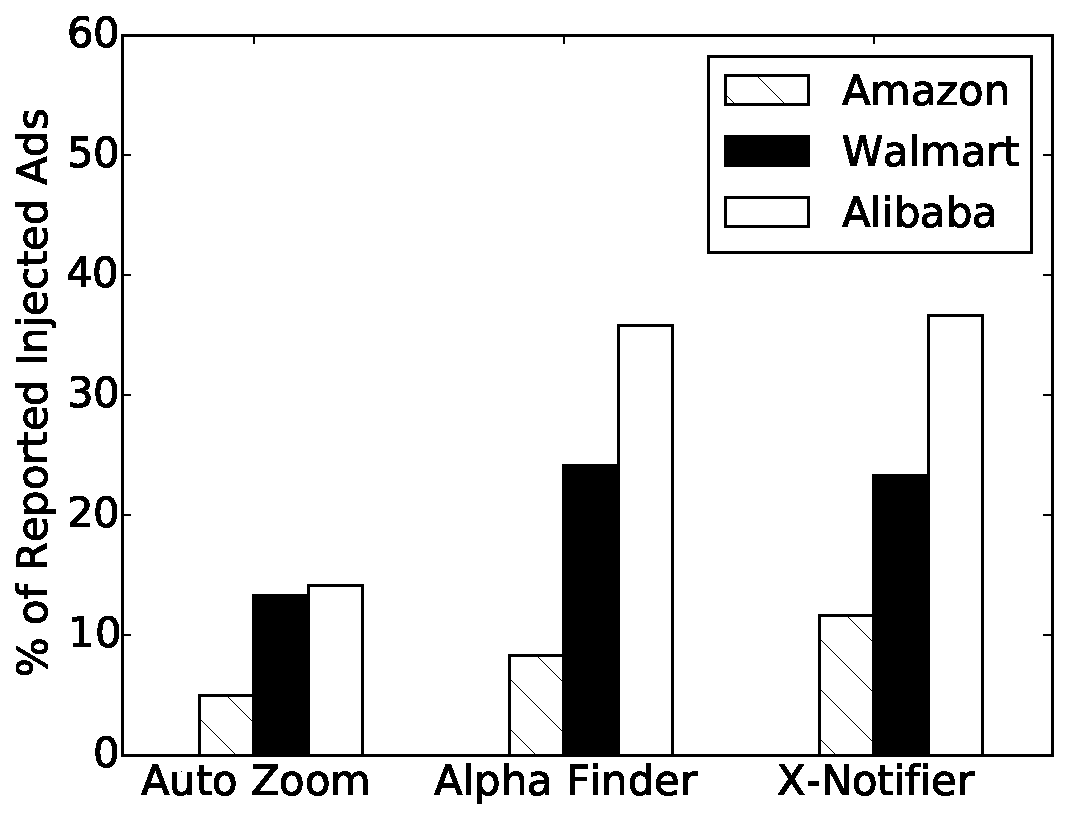
\includegraphics[width=\textwidth]{adinjection/figures/user_study/user_study_1}
        \caption{\scriptsize{Group 1.}}
        \label{adinjection:fig:eval:user_study:1}
    \end{subfigure}
    \hfill
    \begin{subfigure}[t]{0.48\textwidth}
        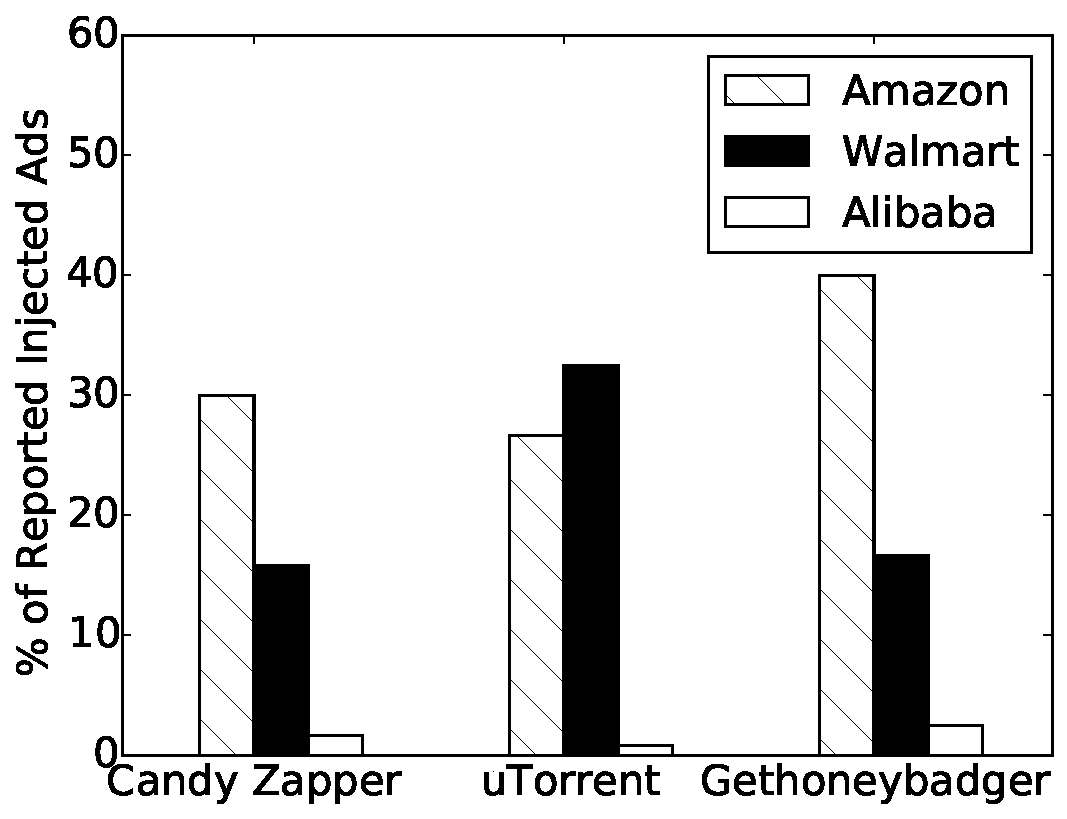
\includegraphics[width=\textwidth]{adinjection/figures/user_study/user_study_2}
        \caption{\scriptsize{Group 2.}}
        \label{adinjection:fig:eval:user_study:2}
    \end{subfigure}
    \caption{Percentage of injected ads that are reported correctly by all the participants.}
    \label{adinjection:fig:eval:extensions_adinjection}
\end{figure}


The goal of the first phase of the experiment was to measure whether users were
able to detect third-party content that was not intended for inclusion by the
publishers of web pages presented to them. Users were divided into two equal
sized groups of 40. In each group, users were first presented with three
unmodified Chromium browsers, each of which had a separate ad-injecting
extension installed. Using each browser, the participants were asked to visit
three popular retail websites.

Each ad-injecting extension monitors for visits to these websites, and each
injects three different types of advertisements into these sites. For each
website, we asked the participants to examine the page and tell us if they
noticed any content in the page that did not belong to the website -- in other
words, whether any content did not seem to originate from the publisher. For
each group, we aggregated the responses and presented the percentage of
correctly reported ad injection incidents for each extension in
Figure~\ref{adinjection:fig:eval:extensions_adinjection}.

We then asked each participant whether they would click on ads in general to
measure the degree of trust that users put into the contents on the publisher's
page. Specifically, we asked participants to rate the likelihood of clicking on
ads on a scale from one to five, where one means that they would never click on
an ad while five means that they would definitely click on an ad. We aggregated
the responses and present the results in
Figure~\ref{adinjection:fig:eval:user_study:susceptibility}.

\begin{figure}[t]
    \centering
    \begin{subfigure}[t]{0.32\textwidth}
        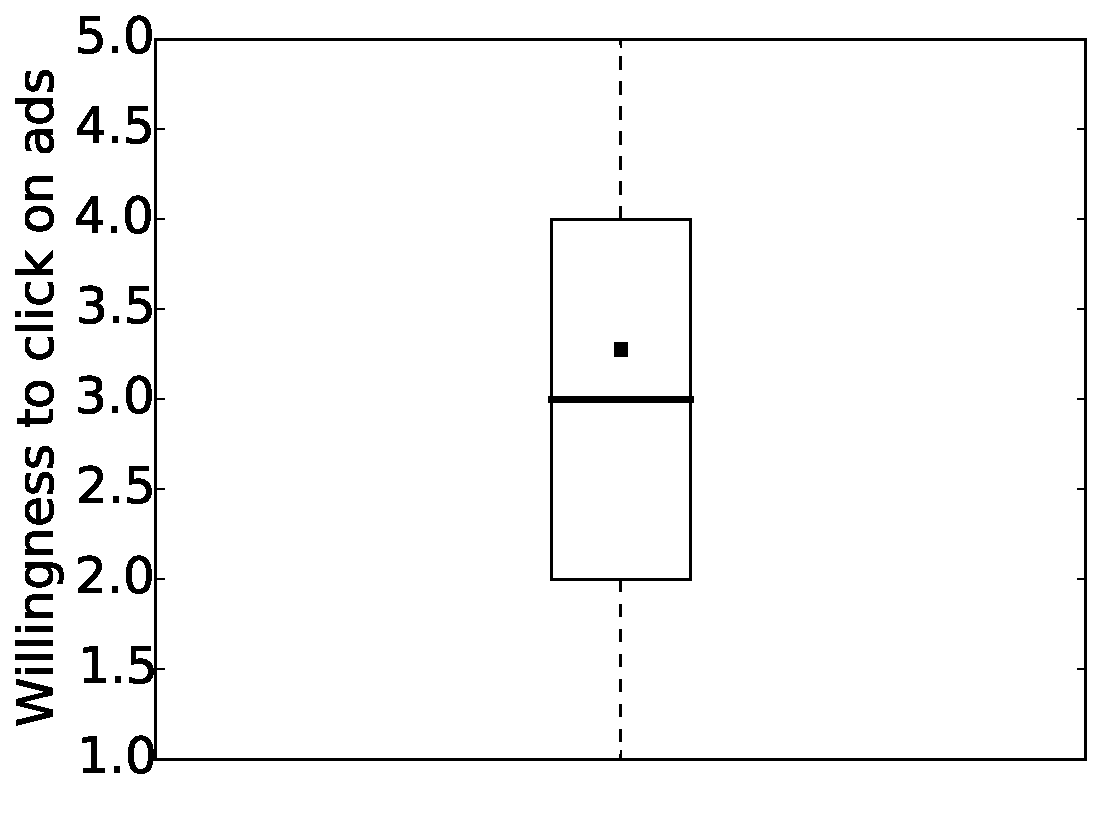
\includegraphics[width=\textwidth]{adinjection/figures/user_study/clicking.pdf}
        \caption{\scriptsize{Susceptibility to ad injection.}}
        \label{adinjection:fig:eval:user_study:susceptibility}
    \end{subfigure}
    \hfill
    \begin{subfigure}[t]{0.32\textwidth}
        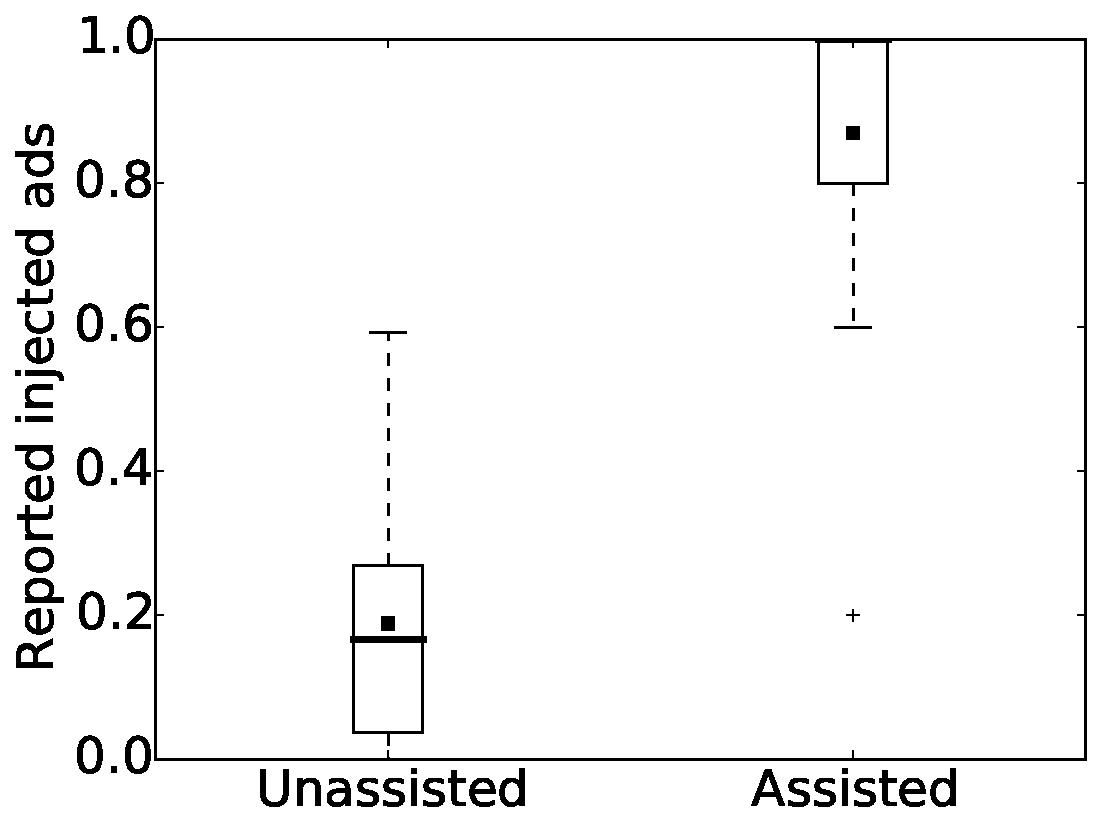
\includegraphics[width=\textwidth]{adinjection/figures/user_study/identification.pdf}
        \caption{\scriptsize{Ability to identify injected ads.}}
        \label{adinjection:fig:eval:user_study:identification}
    \end{subfigure}
    \hfill
    \begin{subfigure}[t]{0.32\textwidth}
        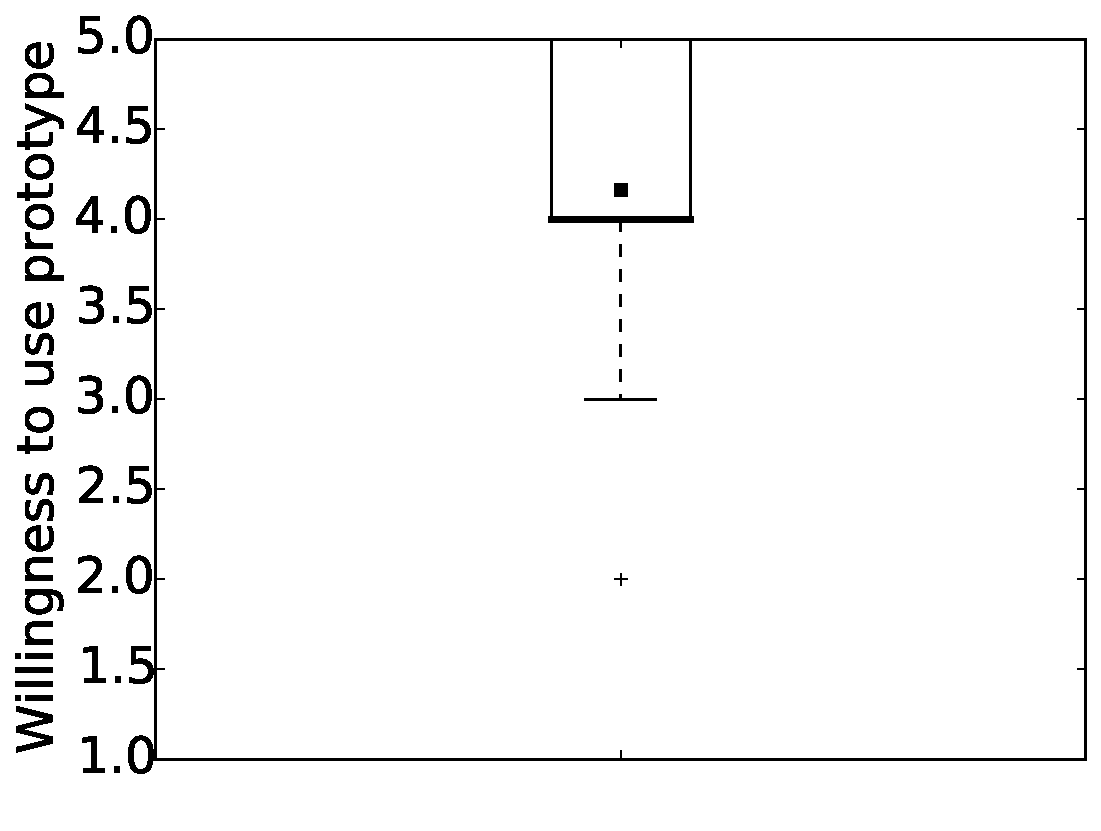
\includegraphics[width=\textwidth]{adinjection/figures/user_study/willingness.pdf}
        \caption{\scriptsize{Usability of content provenance.}}
        \label{adinjection:fig:eval:user_study:usability}
    \end{subfigure}
    \caption{User study results. For each boxplot, the box represents the
    boundaries of the first and third quartiles. The band within each box
    is the median, while the black square is the mean. The whiskers represent
    1.5 IQR boundaries, and outliers are represented as a \texttt{+} symbol.}
    \label{adinjection:fig:eval:user_study}
\end{figure}


\subsubsection{Effectiveness of Content Provenance Indicators}
\label{adinjection:sec:analysis:effectiveness}

After the first phase of the experiment, we briefly explained the purpose of
\origintracer and content provenance to the participants. Then, for each
participant in each group, we picked one of the three ad-injecting extensions in
which, the participant did not detect most of the injected ads and installed it
on a Chromium instance equipped with \origintracer. Then, each participant was
asked to visit one of the three retail websites by his choice and identify
third-party content modifications -- i.e., injected ads -- with the help of
provenance indicators. The results are shown in
Figure~\ref{adinjection:fig:eval:user_study:identification}.

Finally, we asked each participant how likely they would be to use the content
provenance system in their daily web browsing. We asked participants to rate
this likelihood on a scale from one to five, where one means they would never
use the system and five means that they would always use it. The results are
shown in Figure~\ref{adinjection:fig:eval:user_study:usability}.

\subsubsection{Performance}
\label{adinjection:sec:analysis:perf}

To measure the performance overhead of \origintracer, we configured both an
unmodified Chromium browser and the prototype to automatically visit the Alexa
Top 1K. Moreover, we configured both browser instances with the five
high-profile extensions. We built a crawler based on Selenium
WebDriver~\cite{selenium} to automatically visit the entire list of websites and
recorded the total elapsed time from the beginning of the browsing process until
the entire list of websites was visited.

We repeated the experiment 10 times and measured the average elapsed time. The
average elapsed time for browsing the home pages of the Alexa Top 1K websites
measured in this way is 3,457 seconds for the unmodified browser and 3,821
seconds for \origintracer. Therefore, \origintracer incurred a 10.5\% overhead
on browsing time on average.

\subsubsection{Usability}
\label{adinjection:sec:analysis:usability}

We conducted another experiment on 13 students with different technical
background. We presented the participants with \origintracer integrated into
Chromium~43, and asked them to browse the web for several hours, visiting any
websites of their choice. In addition, for each user, we randomly selected 50
websites from the Alexa Top 500 and asked the user to visit them. We also
configured the browser with the five high-profile extensions. We asked
participants to record the number of pages in which they encountered any errors
or broken functionality for the extensions. Out of close to 2,000 URLs, 29
errors were encountered. In addition, none of the participants reported any
broken extensions.
